\setproblem{19701}

\begin{frame}[label=p4]{소 운전한다.(19701)}
\footnotesize

\textbf{문제}

소들은 날아다니는 대신 그냥 운전을 하기로 했다. 대한민국에는 도시가 $V$개 있고,
두 도시를 양방향으로 잇는 고속도로가 $E$개 있다. 모든 소들은 선린인터넷고가 있는
$1$번 도시에 산다. 모든 고속도로의 가운데에는 돈까스를 파는 휴게소가 하나씩 있다.

베시는 다른 도시로 여행을 떠나려 한다. 경로를 잘 골라
$1$번 도시에서 각 도시까지 가는 데 걸리는 시간의 최솟값을 구하려 한다.
즉, $2$번부터 $V$번까지 각 도시까지의 최단 시간을 구하라.

하지만 베시는 휴게소의 돈까스를 먹고 싶어졌다.
각 고속도로의 휴게소에는 돈까스의 맛이 수치로 주어진다.

베시는 여행 경로 중 \textbf{정확히 한 개의 휴게소}에 들러 돈까스를 먹을 것이다.

각 도시 $i$에 대해 다음 값을 최소화하라.

\[
(\text{1번 도시에서 i번 도시까지 이동 시간}) - (\text{먹은 돈까스의 맛})
\]
\end{frame}

\begin{frame}{예제 그래프}

\begin{center}
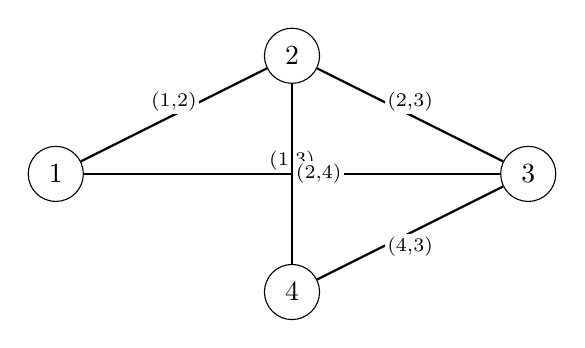
\begin{tikzpicture}[
vertex/.style={circle,draw,minimum size=7mm},
edge/.style={thick},
lab/.style={font=\scriptsize,fill=white,inner sep=1pt}
]

\node[vertex] (1) at (0,0) {1};
\node[vertex] (2) at (3,1.5) {2};
\node[vertex] (3) at (6,0) {3};
\node[vertex] (4) at (3,-1.5) {4};

\draw[edge] (1) -- node[lab,above] {(1,2)} (2);
\draw[edge] (1) -- node[lab,above] {(1,3)} (3);
\draw[edge] (2) -- node[lab,above] {(2,3)} (3);
\draw[edge] (2) -- node[lab,right] {(2,4)} (4);
\draw[edge] (4) -- node[lab,below] {(4,3)} (3);

\end{tikzpicture}
\end{center}

\end{frame}


\begin{frame}[fragile, allowframebreaks]{정의찬 소스 코드}
\inputminted{java}{../src/\prob/uichan/Main.java}
\end{frame}

\begin{frame}[fragile, allowframebreaks]{서민종 소스 코드}
\inputminted{java}{../src/\prob/minjong/Main.java}
\end{frame}

\begin{frame}[fragile, allowframebreaks]{원찬혁1 소스 코드}
\inputminted{java}{../src/\prob/chanhyeok/Main1.java}
\end{frame}

\begin{frame}[fragile, allowframebreaks]{원찬혁2 소스 코드}
\inputminted{java}{../src/\prob/chanhyeok/Main2.java}
\end{frame}

\begin{frame}[fragile, allowframebreaks]{김시온 소스 코드}
\inputminted{java}{../src/\prob/sion/Main.java}
\end{frame}

\begin{frame}{음수 가중치가 있는 그래프에서 데이크스트라}

\begin{center}
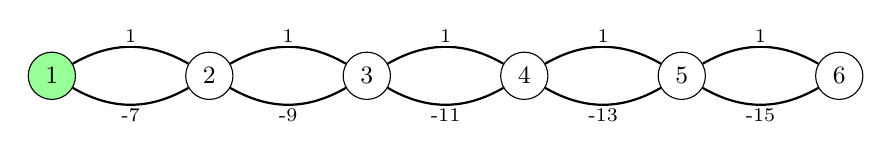
\begin{tikzpicture}[
    vertex/.style={circle, draw, minimum size=6mm, inner sep=0pt, font=\small},
    start/.style={circle, draw, fill=green!40, minimum size=6mm, inner sep=0pt, font=\small},
    edge/.style={thick},
    w/.style={font=\scriptsize, fill=white, inner sep=1pt}
]

% ---- nodes ----
\node[start] (1) at (0,0) {1};
\node[vertex] (2) at (2,0) {2};
\node[vertex] (3) at (4,0) {3};
\node[vertex] (4) at (6,0) {4};
\node[vertex] (5) at (8,0) {5};
\node[vertex] (6) at (10,0) {6};

% ---- edges ----

\draw[edge] (1) to[bend left=30] node[w,above] {1} (2);
\draw[edge] (1) to[bend right=30] node[w,below] {-7} (2);

\draw[edge] (2) to[bend left=30] node[w,above] {1} (3);
\draw[edge] (2) to[bend right=30] node[w,below] {-9} (3);

\draw[edge] (3) to[bend left=30] node[w,above] {1} (4);
\draw[edge] (3) to[bend right=30] node[w,below] {-11} (4);

\draw[edge] (4) to[bend left=30] node[w,above] {1} (5);
\draw[edge] (4) to[bend right=30] node[w,below] {-13} (5);

\draw[edge] (5) to[bend left=30] node[w,above] {1} (6);
\draw[edge] (5) to[bend right=30] node[w,below] {-15} (6);

\end{tikzpicture}
\end{center}

\end{frame}